\section{Auswertung}
\label{sec:Auswertung}

\subsection{Diffferentielle Energieverteilung der Elektronen}

Zu Beginn wird die Messung bei $T=20\,\unit{\celsius}$ ausgewertet.
Die mithilfe des analogen x-y-Schreibers erzeugte Grafik ist in \autoref{fig:Int Energie 20 Grad} dargestellt.
Sie stellt die integrale Energieverteilung der Elektronen dar.

\begin{figure}[H]
  \centering
  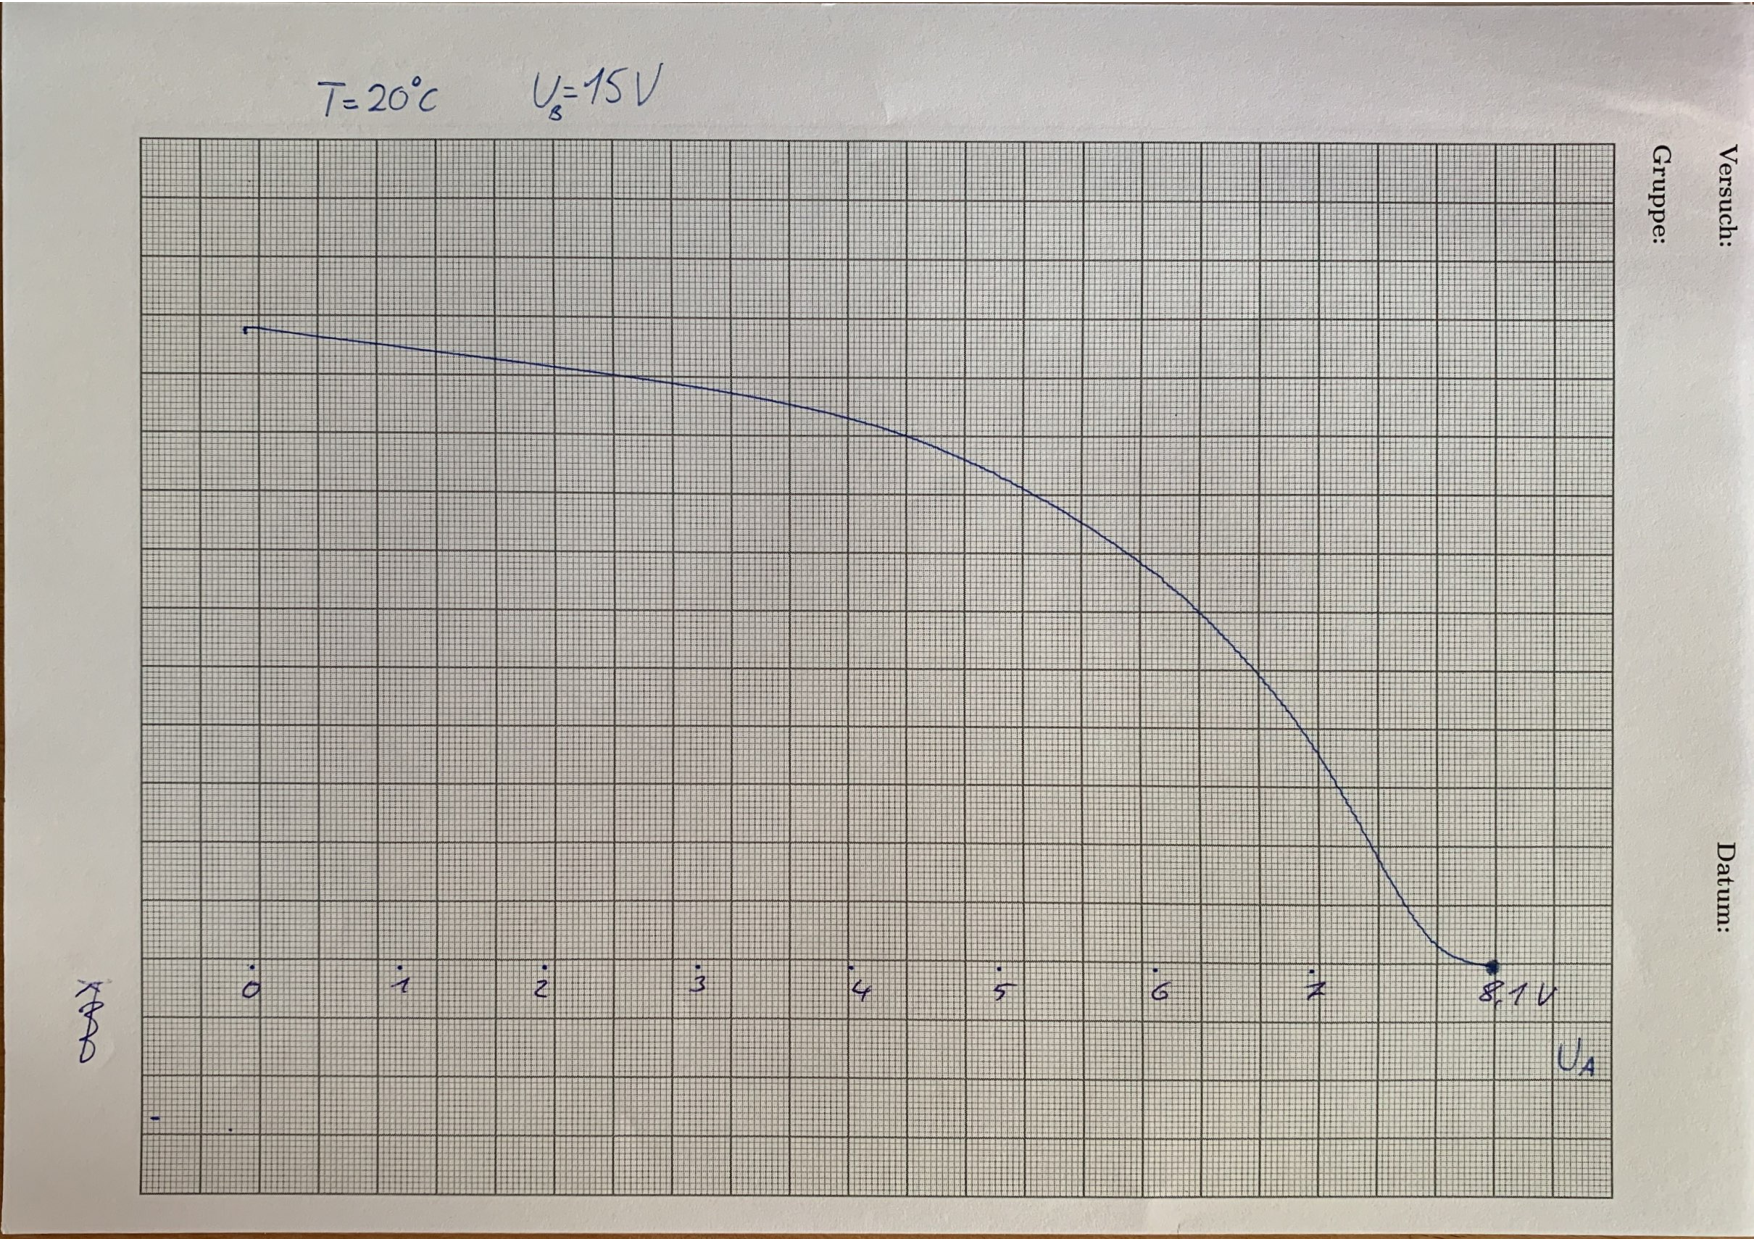
\includegraphics[height=8cm]{content/pics/originaldaten/1.pdf}
  \caption{Aufgezeichnete Integrale Energieverteilung der Elektronen $T=20\,\unit{\celsius}$.}
  \label{fig:Int Energie 20 Grad}
\end{figure}

Um nun die differentielle Energieverteilung der Elektronen zu erhalten, werden an mehreren Werten
für $U_A$ kleine Steigungsdreiecke verwendet.
Deren Länge wird zu $\symup{\Delta}U_{\symup{A}}=0.5\,\unit{\volt}$ gewählt. Dann berechnet sich die lokale
Änderung des Auffängerstroms über die Gleichung
\begin{equation*}
\symup{\Delta}I_{\symup{A}}(U_{\symup{A}})=I_{\symup{A}}(U_{\symup{A}})-I_{\symup{A}}(U_{\symup{A}}+\symup{\Delta}U_{\symup{A}}).
\end{equation*}
Die so ermittelten Wertepaare sind in \autoref{tab:Diff Energie 20 Grad} festgehalten.

\begin{table}[H]
  \centering
  \caption{Abgelesene Wertepaare für $U_{\symup{A}}$ und $\symup{\Delta}I_{\symup{A}}$ aus zehn Steigungsdreiecken in \autoref{fig:Int Energie 20 Grad}}
  \label{tab:Diff Energie 20 Grad}
  \begin{tabular}{S[table-format=1.1] S[table-format=1.1] S[table-format=2.0]}
      \toprule
       {$U_{\symup{A}}\,/\,\unit{\volt}$} & {$\symup{\Delta}U_{\symup{A}}\,/\,\unit{\volt}$} & {$\symup{\Delta}I_{\symup{A}}(U_{\symup{A}})\,/\,\unit{\ampere}$} \\
      \midrule
      0.0 & 0.5 &	3 \\
      0.5 & 0.5 &	2 \\
      1.0 & 0.5 &	2 \\
      1.5 & 0.5 &	1 \\
      2.0 & 0.5 &	2 \\
      2.5 & 0.5 &	2 \\
      3.0 & 0.5 &	2 \\
      3.5 & 0.5 &	3 \\
      4.0 & 0.5 &	4 \\
      4.5 & 0.5 &	6 \\
      5.0 & 0.5 &	7 \\
      5.5 & 0.5 &	9 \\
      6.0 & 0.5 &	12 \\
      6.5 & 0.5 &	18 \\
      7.0 & 0.5 &	23 \\
      7.5 & 0.5 &	14 \\
      \bottomrule 
  \end{tabular}
\end{table}

In \autoref{fig:Diff Energie 20Grad} sind die Werte geplottet, zusammen beschreiben sie den Verlauf der gesuchten differentiellen
Energieverteilung.
Aufgrund der geringen Temperatur finden hier so gut wie keine Wechselwirkungen von Elektronen und Hg-Atomen statt.
Für den Dampfdruck und die mittlere freie Weglänge ergeben sich mit den Formeln \eqref{eq:p_sät} und \eqref{eq:freie weglänge} die Werte
\begin{align*}
  p_{\symup{saet}} &= \qty{0.0036}{\milli\bar} \\
  \bar{w}(T) &= 0,810\,\unit{\centi\meter}.
\end{align*}
Der Abstand $a$ zwischen Kathode und Beschleunigungselektrode wird auf $a\approx\qty{1}{\centi\metre}$ geschätzt und es wird das
Verhältnis $\frac{a}{\bar{w}}$ bestimmt, um eine gute Aussage über die Anzahl der Stöße treffen zu können. Ein großer Wert bedeutet hier, dass
viele Stöße stattfinden. Es folgt
\begin{equation*}
  \frac{a}{\bar{w}} = \num{1,23}.
\end{equation*}
% Die freie Weglänge der Elektronen im Quecksilberdampf beträgt bei dieser Temperatur nach \eqref{eq:freie weglänge}
% $\bar{w}(T) = 0,810\,\unit{\centi\meter}$. Sie ist damit beinahe so lang wie der Abstand zwischen Kathode und
% Beschleunigungselektrode, somit finden nur sehr wenige Stöße statt.

Aus dem Kurvenverlauf lässt sich schließen, dass die Änderung des Auffängerstroms zunächst mit steigendem $U_{\symup{A}}$ zunimmt.
Bei $U_{\symup{A}}=7\,\unit{\volt}$ nimmt sie ihr Maximum an, dannach fällt die Änderung wieder schnell ab.
Dies bedeutet, dass die meisten Elektronen eine Energie im Bereich um $U_{\symup{A}}=7\,\unit{\electronvolt}$ aufweisen.
Eine Erhöhung der Bremsspannung hat in diesem Bereich also einen besonders großen Einfluss auf den Auffängerstrom.

Das Kontaktpotential $K$ berechnet sich somit aus der Differenz der tatsächlichen Beschleunigungsspannung und der des Peaks:
\begin{equation*}
  K=U_{\symup{B}}-U_{\symup{Peak}}=(15-7)\,\unit{\volt}=8\,\unit{\volt}
\end{equation*}

\begin{figure}[H]
    \centering
    \includegraphics[height=8cm]{build/Differentielle_Energie_20Grad.pdf}
    \caption{Differentielle Energieverteilng der Elektronen bei $T=20\,\unit{\celsius}$.}
    \label{fig:Diff Energie 20Grad}
\end{figure}

Die Auswertung der Messreihe für $T=145\,\unit{\celsius}$ erfolgt analog zur niedrigen Temperatur.

\begin{figure}[H]
  \centering
  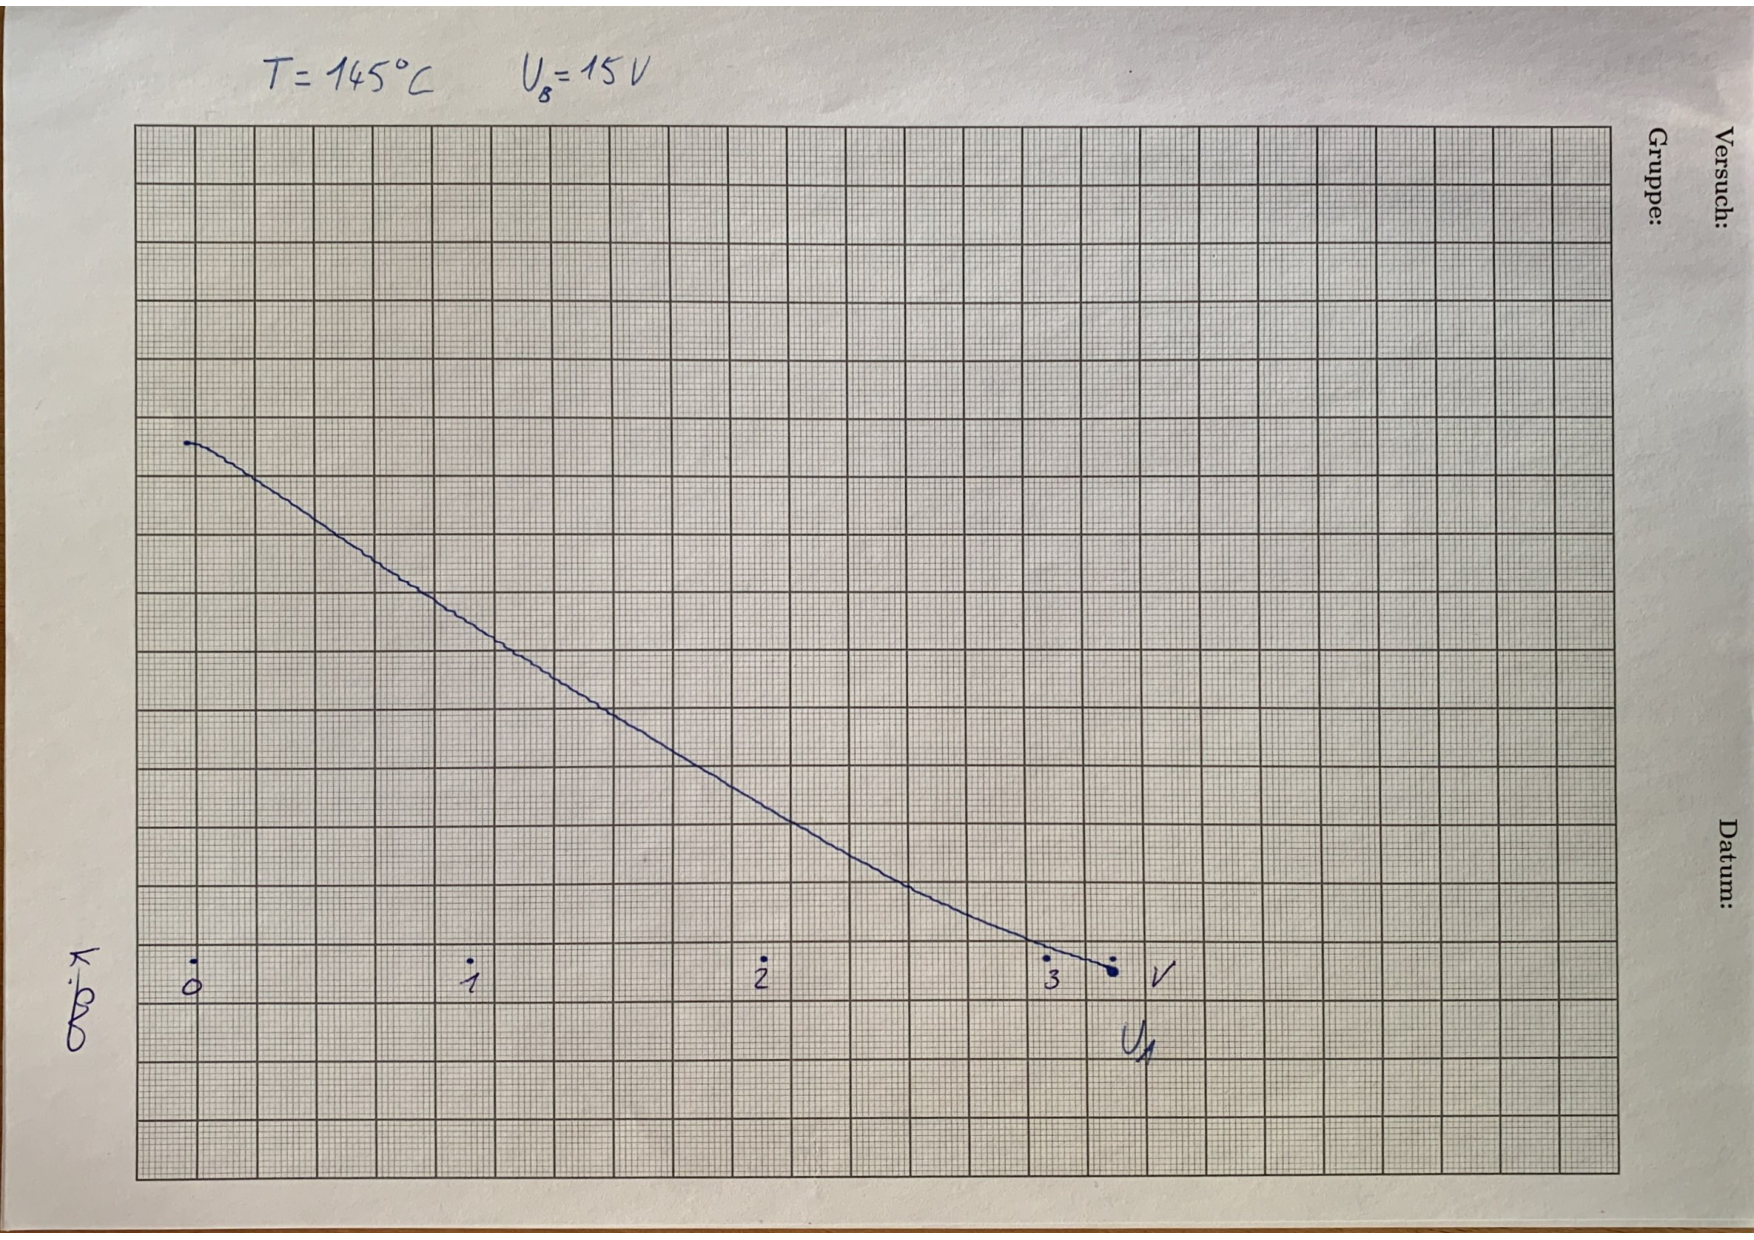
\includegraphics[height=8cm]{content/pics/originaldaten/2.pdf}
  \caption{Aufgezeichnete Integrale Energieverteilung der Elektronen $T=145\,\unit{\celsius}$.}
  \label{fig:Int Energie 145 Grad}
\end{figure}

\begin{table}[H]
  \centering
  \caption{Abgelesene Wertepaare für $U_A$ und $\symup{\Delta}I_A$ aus 4 Steigungsdreiecken in \autoref{fig:Int Energie 145 Grad}}
  \label{tab:Diff Energie 145 Grad}
  \begin{tabular}{S[table-format=1.1] S[table-format=1.1] S[table-format=2.0]}
      \toprule
       {$U_{\symup{A}}\,/\,\unit{\volt}$} & {$\symup{\Delta}U_{\symup{A}}\,/\,\unit{\volt}$} & {$\symup{\Delta}I_{\symup{A}}(U_{\symup{A}})\,/\,\unit{\ampere}$} \\
      \midrule
      0.0 & 0.5 &	15 \\
      0.5 & 0.5 &	15 \\
      1.0 & 0.5 &	16 \\
      1.5 & 0.5 &	17 \\
      2.0 & 0.5 &	14 \\
      \bottomrule 
  \end{tabular}
\end{table}


\begin{figure}[H]
    \centering
    \includegraphics[height=8cm]{build/Differentielle_Energie_145Grad.pdf}
    \caption{Differentielle Energieverteilng der Elektronen bei $T=145\,\unit{\celsius}$.}
    \label{fig:Diff Energie 145Grad}
\end{figure}

Hier fällt der Auffängerstrom schnell auf Null ab, die Steigung ist dabei nahezu konstant.
Aufgrund der deutlich höheren Temperatur können viele elastische Stöße
zwischen den Elektronen und Hg-Atomen stattfinden. Dabei werden die Elektronen gestreut und besitzen nur noch
eine geringe kinetische Energie in z-Richtung.
Dies lässt sich durch die geringe freie Weglänge bestätigen, die legiglich $\bar{w}(T) = 7,303\,\unit{\micro\meter}$ beträgt.
Der Dampfdruck und das Verhältnis $\frac{a}{\bar{w}}$ bestimmen sich zu
\begin{align*}
  p_{\symup{saet}} &= \qty{3.97}{\milli\bar} \\
  \frac{a}{\bar{w}} &= \num{1369}.
\end{align*}

\subsection{Franck-Hertz-Kurve}
\label{sec:Franck-Hertz-Kurve}

Zur Bestimmung der Anregungsenergie der Hg-Atome werden die zwei aufgezeichneten Kurven getrennt ausgewertet.
Entscheidend sind die relativen Abstände der Peaks zueinander, deren Mittelwert entspricht direkt der
gesuchten Anregungsenergie. Die erste Kurve ist in \autoref{fig:FHZ 166Grad} dargestellt.
Für den Dampfdruck, die mittlere freie Weglänge, und das Verhältnis $\frac{a}{\bar{w}}$ ergibt sich
\begin{align*}
  p_{\symup{saet}} &= \qty{8.72}{\milli\bar} \\
  \bar{w}(T) &= \qty{3.33}{\micro\meter} \\
  \frac{a}{\bar{w}} &= \num{3006}.
\end{align*}

\begin{figure}[H]
  \centering
  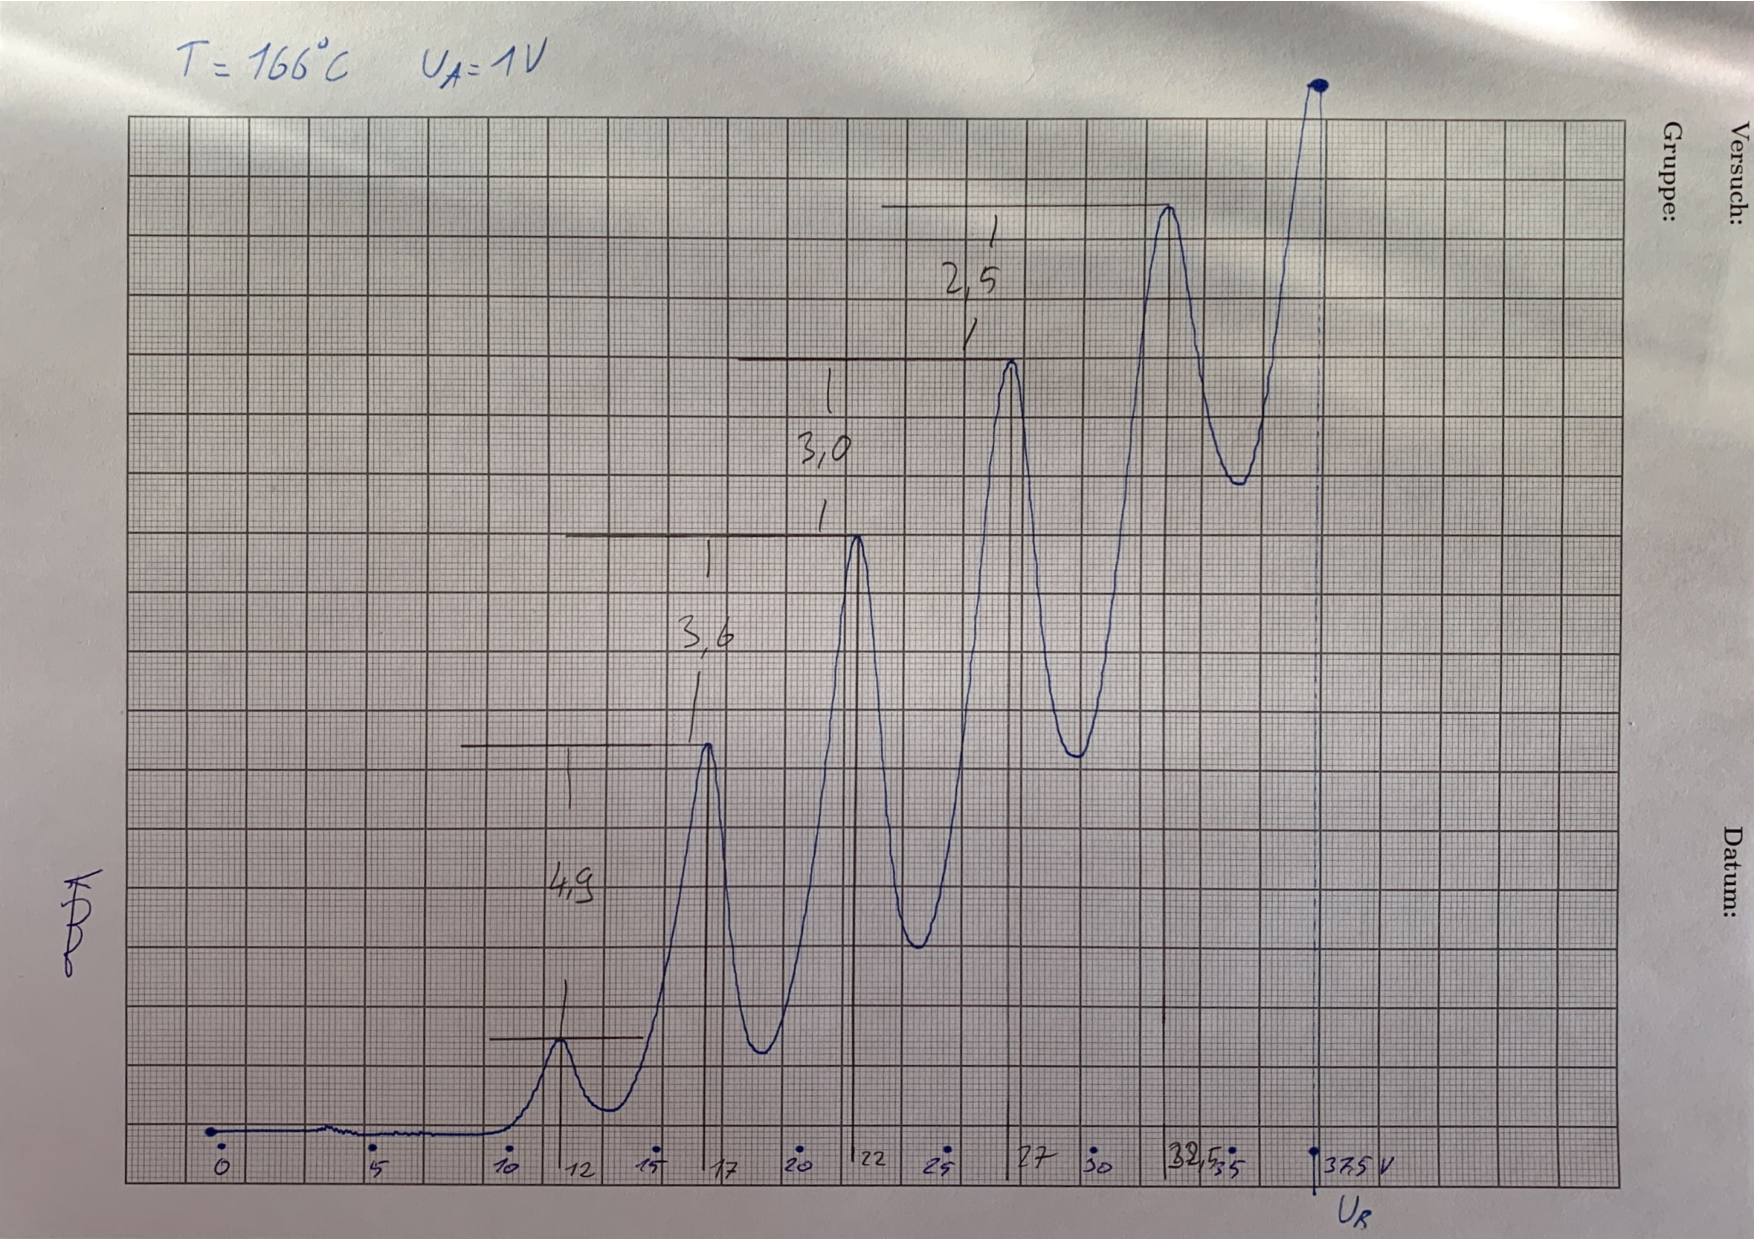
\includegraphics[height=8cm]{content/data/FH_166.pdf}
  \caption{Aufgezeichnete Franck-Hertz Kurve bei $T=166\,\unit{\celsius}$.}
  \label{fig:FHZ 166Grad}
\end{figure}

Die jeweiligen Abstände der Peaks sind beretis auf der x-Achse vermerkt, somit muss nur noch deren
Mittelwert bestimmt werden. Mithilfe der Python Erweiterung \textit{uncertainties}~\cite{uncertainties} 
ergibt sich als Ergebnis der ersten Versuchsreihe:
\begin{gather*}
    \bar{E_1}=\qty{5.12+-0.22}{\electronvolt}.
\end{gather*}
Mithilfe von \eqref{eq:Einstein ist smart} wird berechnet sich die Wellenlänge der beim Übergang in den
Grundzustand emittierten Strahlung zu:
\begin{gather*}
  \lambda_1=\qty{242+-10}{\nano\meter}.
\end{gather*}

Für die zweite Messreihe wird identisch vorgegangen, die zugehörige Frank-Hertz Kurve ist in \autoref{fig:FHZ 195Grad} zu sehen.
Die Werte für Dampfdruck, freie Weglänge, und das Verhältnis $\frac{a}{\bar{w}}$ ergeben sich hier zu
\begin{align*}
  p_{\symup{saet}} &= \qty{22.99}{\milli\bar} \\
  \bar{w}(T) &= \qty{1.26}{\micro\meter} \\
  \frac{a}{\bar{w}} &= \num{7929}.
\end{align*}

\begin{figure}[H]
  \centering
  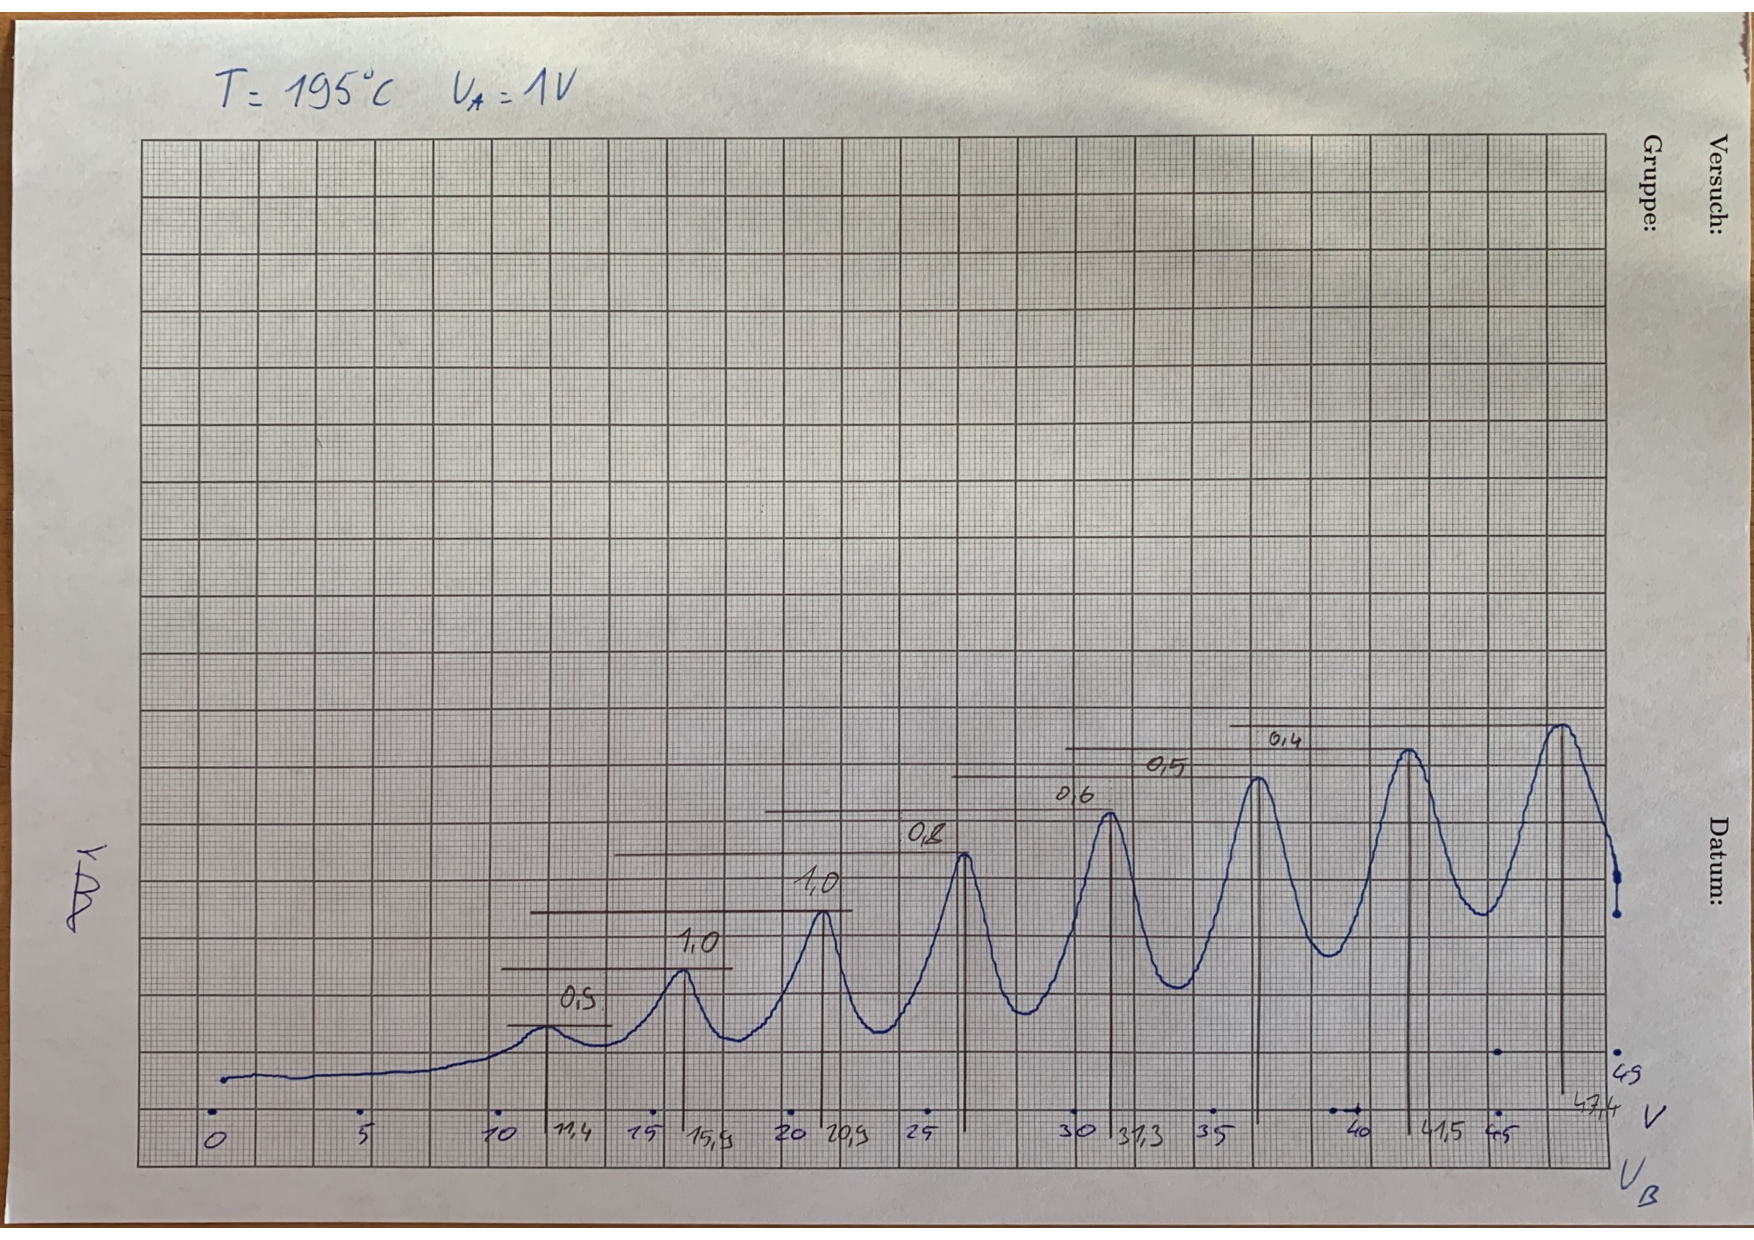
\includegraphics[height=8cm]{content/data/FH_195.pdf}
  \caption{Aufgezeichnete Franck-Hertz Kurve bei $T=195\,\unit{\celsius}$.}
  \label{fig:FHZ 195Grad}
\end{figure}

Es ergibt sich hier abschließend:
\begin{gather*}
  \bar{E_2}=\qty{5.1+-0.4}{\electronvolt}
\end{gather*}
sowie eine Wellenlänge von
\begin{gather*}
  \lambda_2=\qty{241+-18}{\nano\meter}.
\end{gather*}

Die elastischen Stöße der Elektronen haben keinen Einfluss auf das Ergebnis, da sie lediglich aufgrund des
Energienverlustes die Höhe der Franck-Hertz Kurve beeinflussen. Die relativen Abstände der Peaks bleiben 
davon unverändert.